% Figure 1: the XAI-SDN system architecture, drawn as vector TikZ.
% The entropy module carries the qualified complexity claim (expected
% amortized O(1)) so the figure agrees with the abstract, Sec. II-A,
% Sec. IV, Sec. V-C and the Fig. 2 caption.
% All six control-plane modules share one text width so the two rows form
% a regular grid and no label overhangs its box or the controller frame.
\documentclass[tikz,border=4pt]{standalone}
\usepackage{amsmath,amssymb}
\usepackage{xcolor}
\usetikzlibrary{shapes.geometric, arrows.meta, positioning, fit, backgrounds, calc}

\definecolor{xsdnblue}{RGB}{0,114,178}
\definecolor{xsdnteal}{RGB}{0,158,115}
\definecolor{xsdnorange}{RGB}{230,159,0}
\definecolor{xsdnred}{RGB}{213,94,0}
\definecolor{xsdngray}{RGB}{153,153,153}
\definecolor{cmlow}{RGB}{240,248,255}

\begin{document}
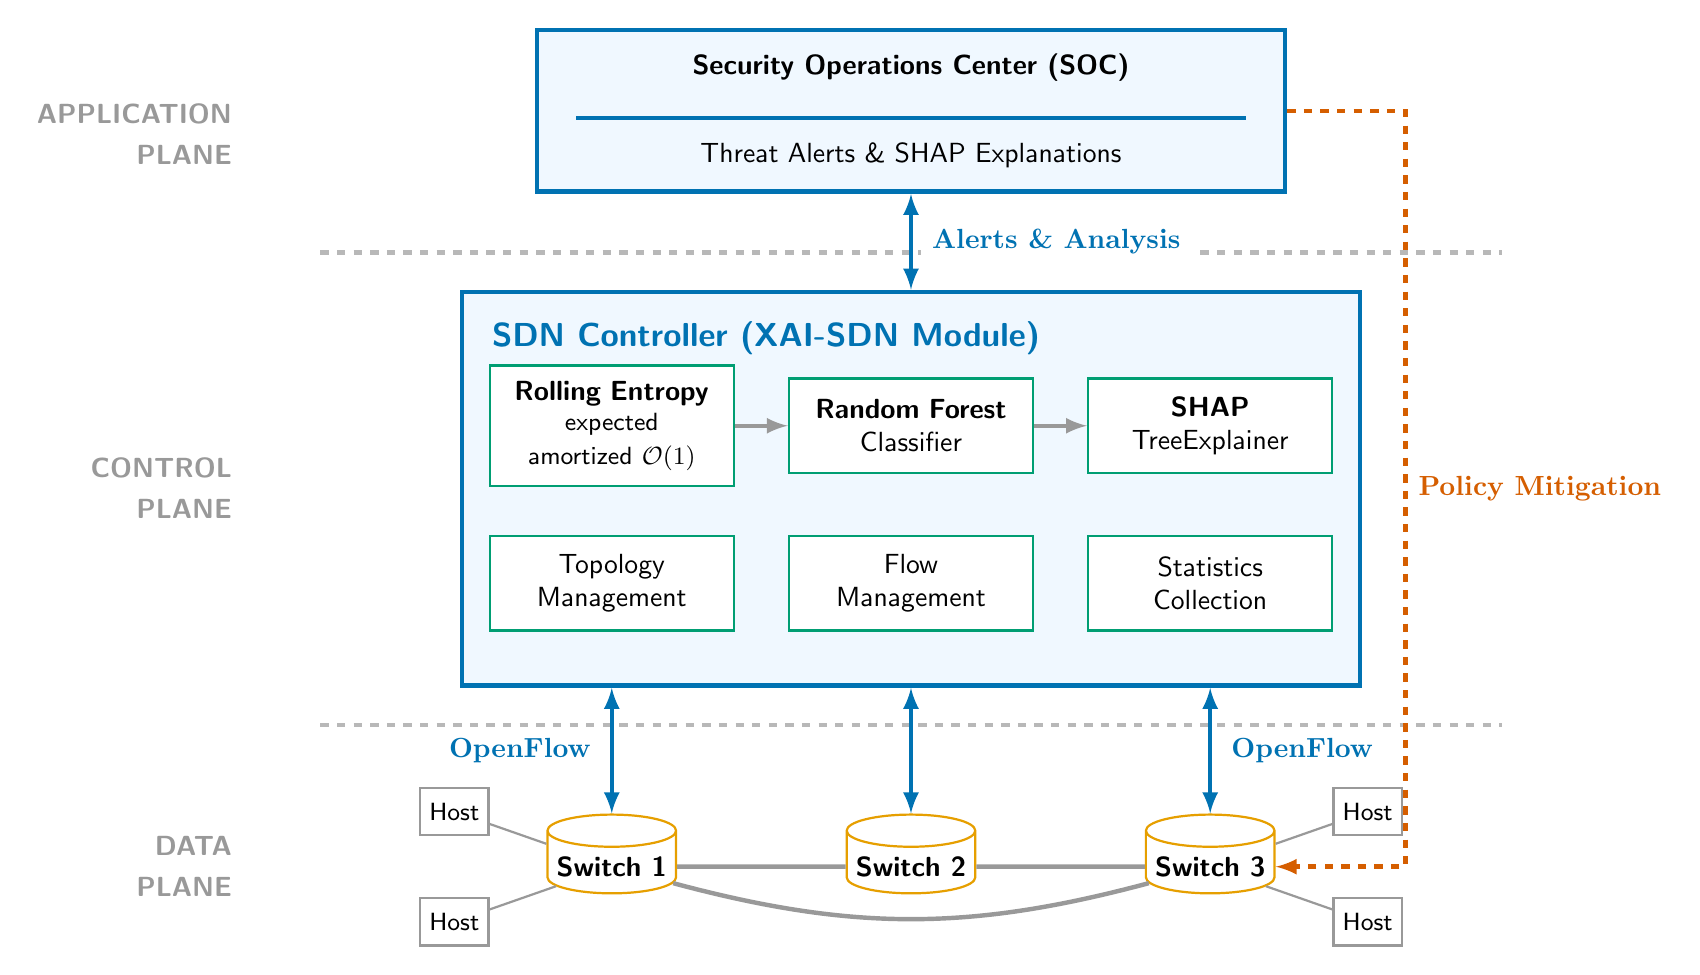
\begin{tikzpicture}[
    font=\sffamily\small,
    >=latex,
    % Styles for professional academic look
    plane/.style={font=\sffamily\bfseries\normalsize, text=xsdngray, align=right, anchor=east},
    planeline/.style={dashed, draw=xsdngray!70, ultra thick},
    controllerbox/.style={draw=xsdnblue, ultra thick, fill=cmlow, align=center},
    module/.style={draw=xsdnteal, thick, fill=white, align=center, inner sep=2mm, minimum height=1.2cm, text width=2.7cm, font=\sffamily},
    dashboard/.style={draw=xsdnblue, ultra thick, fill=cmlow, align=center, inner sep=3mm, minimum width=9.5cm},
    switch/.style={draw=xsdnorange, thick, fill=white, cylinder, shape border rotate=90, aspect=0.25, minimum width=1.6cm, minimum height=1cm, align=center, font=\sffamily\bfseries},
    host/.style={draw=xsdngray, thick, fill=white, rectangle, minimum width=0.8cm, minimum height=0.6cm, align=center, font=\sffamily\small},
    arrow/.style={->, ultra thick, draw=xsdngray},
    openflow/.style={<->, ultra thick, draw=xsdnblue},
    mitigation/.style={->, dashed, ultra thick, draw=xsdnred}
]

% ----------------------------------------------------
% Horizontal Plane Dividers
% ----------------------------------------------------
\draw[planeline] (-4.5, 3.0) -- (10.5, 3.0);
\draw[planeline] (-4.5, -3.0) -- (10.5, -3.0);

% Plane Labels
\node[plane] at (-5.5, 4.5) {APPLICATION\\[1mm]PLANE};
\node[plane] at (-5.5, 0) {CONTROL\\[1mm]PLANE};
\node[plane] at (-5.5, -4.8) {DATA\\[1mm]PLANE};

% ----------------------------------------------------
% APPLICATION PLANE
% ----------------------------------------------------
\node[dashboard] (dash) at (3, 4.8) {
    \textbf{\normalsize Security Operations Center (SOC)}\\[2mm]
    \textcolor{xsdnblue}{\rule{8.5cm}{1.5pt}}\\[1.5mm]
    \normalsize Threat Alerts \& SHAP Explanations
};

% ----------------------------------------------------
% CONTROL PLANE
% ----------------------------------------------------
% Main SDN Controller Box.  Width 11.4cm spans x in [-2.7, 8.7], which leaves a
% 0.35cm margin around the 3.1cm-wide module boxes centred at -0.8, 3 and 6.8.
\node[controllerbox, minimum width=11.4cm, minimum height=5cm] (controller) at (3, 0) {};
\node[anchor=north west, font=\sffamily\bfseries\large, text=xsdnblue, inner sep=4mm] at (controller.north west) {SDN Controller (XAI-SDN Module)};

% Machine Learning Pipeline.  All six modules share one text width so the two
% rows form a regular grid and no label can overhang its own box.
\node[module] (entropy) at (-0.8, 0.8) {\textbf{Rolling Entropy}\\{\small expected\\amortized $\mathcal{O}(1)$}};
\node[module] (rf) at (3, 0.8) {\textbf{Random Forest}\\Classifier};
\node[module] (shap) at (6.8, 0.8) {\textbf{SHAP}\\TreeExplainer};

\draw[arrow] (entropy) -- (rf);
\draw[arrow] (rf) -- (shap);

% Core Controller Functions
\node[module] (topo) at (-0.8, -1.2) {Topology\\Management};
\node[module] (flow) at (3, -1.2) {Flow\\Management};
\node[module] (stat) at (6.8, -1.2) {Statistics\\Collection};

% ----------------------------------------------------
% DATA PLANE
% ----------------------------------------------------
% OpenFlow Switches
\node[switch] (sw1) at (-0.8, -4.8) {Switch 1};
\node[switch] (sw2) at (3, -4.8) {Switch 2};
\node[switch] (sw3) at (6.8, -4.8) {Switch 3};

\draw[ultra thick, draw=xsdngray] (sw1) -- (sw2);
\draw[ultra thick, draw=xsdngray] (sw2) -- (sw3);
\draw[ultra thick, draw=xsdngray] (sw1) to[bend right=15] (sw3);

% Hosts
\node[host] (h1) at (-2.8, -4.1) {Host};
\node[host] (h2) at (-2.8, -5.5) {Host};
\draw[thick, draw=xsdngray] (h1) -- (sw1);
\draw[thick, draw=xsdngray] (h2) -- (sw1);

\node[host] (h3) at (8.8, -4.1) {Host};
\node[host] (h4) at (8.8, -5.5) {Host};
\draw[thick, draw=xsdngray] (h3) -- (sw3);
\draw[thick, draw=xsdngray] (h4) -- (sw3);

% ----------------------------------------------------
% VERTICAL CONNECTIONS & PROTOCOLS
% ----------------------------------------------------
% OpenFlow Interfaces
% Using "fill=white" to cleanly overwrite the dashed planeline
\draw[openflow] (sw1.north) -- (sw1.north |- controller.south)
    node[midway, left, text=xsdnblue, font=\bfseries\normalsize, fill=white, inner sep=4pt, xshift=-1mm] {OpenFlow};
\draw[openflow] (sw2.north) -- (sw2.north |- controller.south);
\draw[openflow] (sw3.north) -- (sw3.north |- controller.south)
    node[midway, right, text=xsdnblue, font=\bfseries\normalsize, fill=white, inner sep=4pt, xshift=1mm] {OpenFlow};

% Northbound API
\draw[openflow] (controller.north) -- (dash.south)
    node[midway, right, text=xsdnblue, font=\bfseries\normalsize, fill=white, inner sep=4pt, xshift=1mm] {Alerts \& Analysis};

% Feedback Loop (Mitigation)
\draw[mitigation] (dash.east) -- ++(1.5,0) |- (sw3.east)
    node[pos=0.25, right, text=xsdnred, font=\bfseries\normalsize, fill=white, inner sep=4pt] {Policy Mitigation};

\end{tikzpicture}

\end{document}
